%************************************************
\chapter{Black-box Model}\label{ch:Blackbox}
%************************************************

We refer to something as a black-box model when we the user are not aware of the inner workings of the system, like the name suggests we are
in the dark on how the system works, for all we know is that given a by us defined input a black-box transform that into a result according to 
what the system is suppose to do. 

One of the more prominent example for a black-box system are neural networks, they start of with a problem
and exampels on how to solve them, during multiple iterations the network improves itself and is able to solve the problem its designed for
more efficiently and accurately. While we are aware on what the neural network is solving, if we would step into the
code wo wouldnt be able to understand the structure and reasoning behind the decisions and how the neurons interact with one another 
\cite{NeuralNetworks}.

Since we do however compare black-box and white-box model with each other we need to do that on the same systems, therefore
we cannot choose black-box system for our experiments, since if we would do so the white-box model would not be able to any produce data.
We solve this problem by choosing a commonly available white-box system, such as xz, but even though we have acess to the code we dont use
that knowledge and look at the system from a black-box view.

\section{Disadvantages of black-box model}
When using the black-box model we encouter two main challanges, which are combinatorial explosion and collinear features, both need to be
dealed with carefully to produce accurate performance-influence model.

\paragraph{Combinatorial Explosion}
One of the bigger problems we have to deal with when using black-box model is the issue of combinatorial explosion ,which refers to the
effect whereas with a linear increase of features the ammount of possible configuration and therefore variants increase exponentially 
\cite{Combinatorial-explosion}.

Lets assume we have a configurable system whereas each feature is a binary option, that you can either turn on or off. We also define 
that in this system every feature is completly independent from another, i.e. the system got no constraints and turning a feature on or off
does not affect other features. The ammonunt of unique variants that this system would be able to produce is $2^n$, whereas $2$ refers to
the kind feature options we allow, in our case binary and $n$ to the ammount of features. In Figure \ref{fig:Combinatorial-Explosion-Graph}
we can see the effect of combinatorial explosion in such a system, given our system provides 15 features we can see that the ammount of 
unique variants equal to $32768$. 

\begin{figure}[h]
    \centering
    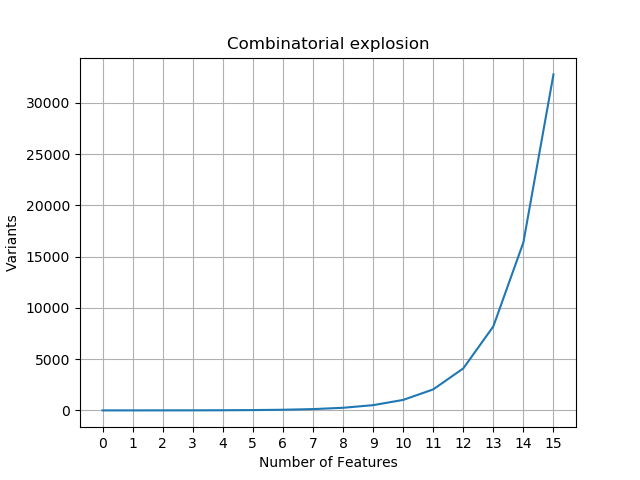
\includegraphics[scale=0.6]{gfx/Combinatorial_explosion_graph.png}
    \caption{Combinatorial Explosion Graph}
    \label{fig:Combinatorial-Explosion-Graph}
\end{figure}

This is where the problem lies, 15 features is by all means not many compared to the ammount of features a real world systems such as the
linux cernel contain. Now all of these different features might interact differently with each other and surely for very small systems
we can brute-force our way by benchmarking every possible variant, however this does not scale, its already unfeasible for systems that
got more then 16 features and therefore over $100.000$ variants. As a reason we cannot completly inspect the whole configuration space and
therefore need to select a subset that represent the system with a high accuracy. To do that state of the art black-box model use sampling
strategies to find a suitable subset, such as, pair-wise sampling, most-enabled-disabled and random sampling. A in depht comparison
between state of the art sampling strategies can be found here \cite{sampling-strategies}.

\paragraph{Colinear Features}
Another problem for our black-box model arises when we have features that are correlated with one another, we call such features collinear.
Lets make a example and revisit our code from Chapter \ref{ch:performance-influence-models} Algorithm \ref{alg:performanceExample} and lets extend
it with the condition $c \leftrightarrow d$. We insert this new condition from Algorithm \ref{alg:Colinear} in Algorithm 
\ref{alg:performanceExample} after line 2.

\begin{algorithm}
    \caption{Colinear Features \label{alg:Colinear}}
    \begin{algorithmic}[1]

    \If{$(c \textit{ and }  \lnot d) or (\lnot c \textit{ and } d)$} 
        \State $c,d \gets False$
    \EndIf

    \end{algorithmic}
    \end{algorithm}

Now if our configuration does not contain c and d the code in line 9 and 11 is unreachable. These colinear features make it hard for our
black-box model to attribute the time correctly to each feature, because if we are unaware of the inner workings we might mistakenly think
that the time increasement when feature c and d is activated is due to the interaction between them, however in reality we see in line
15 that they do not interact at all.